\section{Probability calibration}
The frozen approach applies Platt (sigmoid) calibration to each model. In T06, base predictions were cross-fitted on development folds; each outer training partition generated inner out-of-fold scores for calibration, and the outer validation fold did not fit its model or calibrator. The final bundle fits the Platt mapping to fresh cross-fitted development scores and refits the base estimator on eligible development rows. Thresholds maximize specificity subject to a development sensitivity constraint of at least 0.80; this is a prespecified operating-point assumption, not a universal clinical threshold. Thresholds are 0.15333596 (death), 0.16286458 (ZSN), and 0.07103629 (FIBR\_PREDS). No threshold is used in the probability export.

Table~\ref{tab:development-cal} compares raw and fold-local Platt probabilities on the same 1,360 outer-OOF development records. Platt improved Brier and log loss slightly for death and ZSN; for FIBR\_PREDS both worsened slightly, while Platt remained the frozen assignment-required calibration method. These are development metrics, not test metrics.
\begin{table}[H]\centering\small
\caption{Development OOF probability scores before and after fold-local Platt calibration.}\label{tab:development-cal}
\begin{tabular}{lrrrr}\toprule
Target & Raw Brier & Platt Brier & Raw log loss & Platt log loss\\\midrule
Death & .077211 & .074604 & .262351 & .253899\\
ZSN & .147352 & .146906 & .466140 & .464788\\
FIBR\_PREDS & .082854 & .083415 & .292421 & .294540\\\bottomrule
\end{tabular}\end{table}

The reliability plots in Figure~\ref{fig:devcal} use T06 outer OOF development predictions and quantile bins; they visualize raw versus fold-local Platt scores. Figure~\ref{fig:testcal} is separate and shows the frozen Platt predictions on the final test partition. T07 reports ten-bin equal-width ECE, along with descriptive joint calibration intercept/slope; none of these test diagnostics refits the frozen calibrator.
\begin{figure}[H]\centering
\begin{subfigure}{.32\linewidth}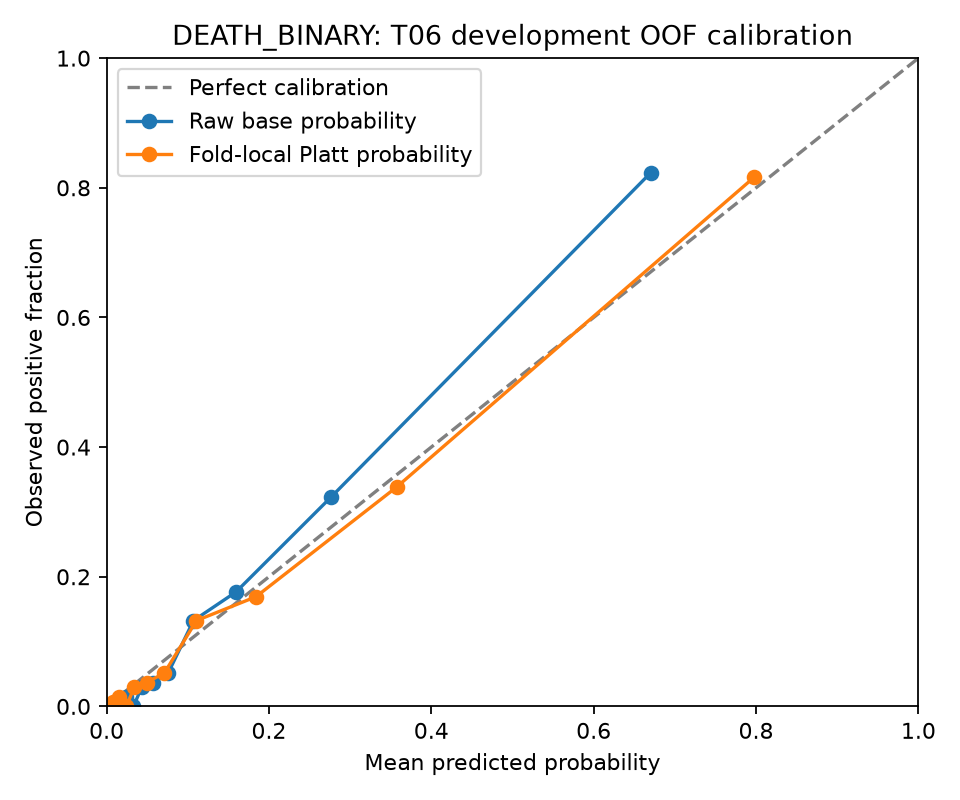
\includegraphics[width=\linewidth]{development_death_binary_raw_vs_platt_reliability.png}\caption{Death}\end{subfigure}
\begin{subfigure}{.32\linewidth}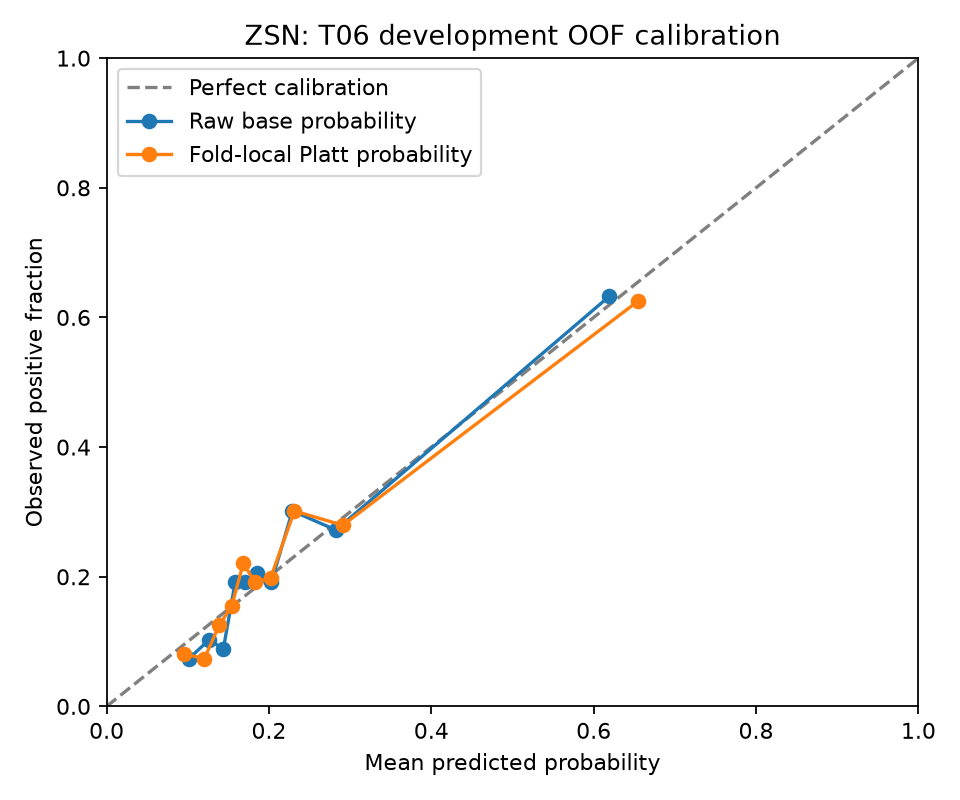
\includegraphics[width=\linewidth]{development_zsn_raw_vs_platt_reliability.png}\caption{ZSN}\end{subfigure}
\begin{subfigure}{.32\linewidth}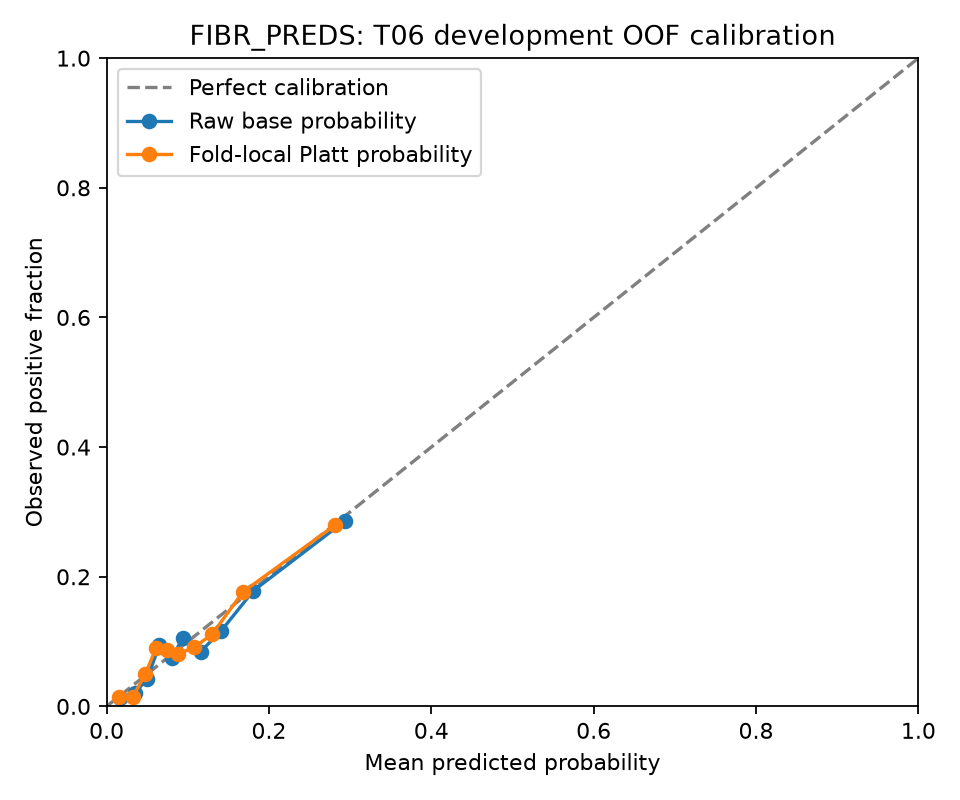
\includegraphics[width=\linewidth]{development_fibr_preds_raw_vs_platt_reliability.png}\caption{FIBR\_PREDS}\end{subfigure}
\caption{Development outer-OOF reliability comparisons. Source: T07 development comparison plots, based on T06 OOF data.}\label{fig:devcal}
\end{figure}
